
\section{Method}
Given a \textit{small} set of expert demonstrations that contain complex robot skill trajectories, we want to learn a visuomotor policy $\pi: \mathcal{O}\mapsto\mathcal{A}$ that maps the visual observations $o\in \mathcal{O}$ to actions $a\in \mathcal{A}$, such that our robots not only reproduce the skill but also generalize beyond the training data. To this end, we introduce \textbf{\oursfull}, which mainly consists of two critical parts: (a) \textbf{Perception.} \ours perceives the environments with point cloud data and processes these visual observations with an efficient point encoder into visual features; (b) \textbf{Decision.} \ours utilizes the expressive Diffusion Policy~\citep{chi2023diffusion_policy} as the action-making backbone, which generates action sequences conditioning on our 3D visual features. An overview of \ours is in Figure~\ref{fig:method}. We will detail each part in the following sections.



\subsection{A Motivating Example}
To better illustrate the generalization ability of \ours, we first give a straightforward example. We use the MetaWorld Reach task~\citep{yu2020metaworld} as our testbed. In this task, the goal is for the gripper to accurately reach a designated target point. To evaluate the effectiveness of imitation learning algorithms in not only fitting training data but also generalizing to new scenarios, we visualize the \textcolor{deepred}{$\bullet$} training points and the \textcolor{deepblue}{$\bullet$} successful evaluation points in 3D space, as shown in Figure~\ref{fig:motivation example}. We observe that with merely five training points, \ours reaches points distributed over the 3D space, while for 2D-based methods, Diffusion Policy~\citep{chi2023diffusion_policy} and IBC~\citep{florence2022ibc} learn to reach within a plane-like area, and  BCRNN~\citep{mandlekar2021robomimic} fails to cover the space. This example demonstrates the superior generalization and efficiency of \ours, particularly in scenarios where available data is limited.

\begin{figure}[htbp]
    \centering
    \vspace{-0.05in}
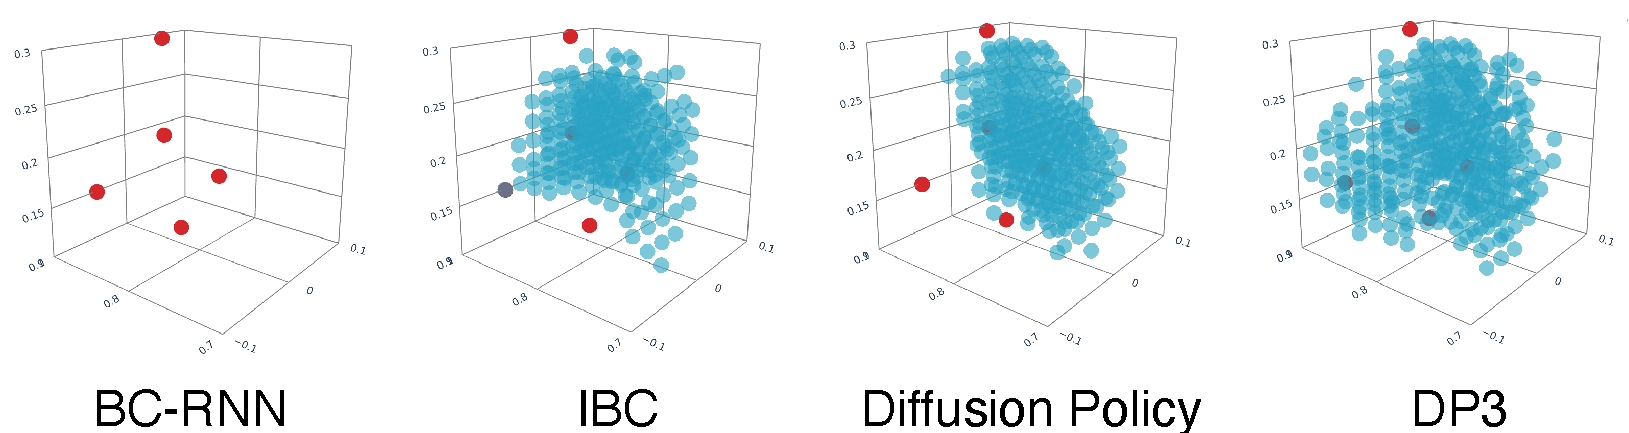
\includegraphics[width=0.5\textwidth]{figures/example.pdf}
    \caption{\textbf{Generalization in 3D space with few data.} We use MetaWorld Reach as an example task, given only 5 demonstrations (visualized by  \textcolor{deepred}{$\bullet$}). We evaluate 1000 times to cover the 3D space and visualize the \textcolor{deepblue}{$\bullet$} successful evaluation points. \textbf{\ours} learns the generalizable skill in 3D space; \textbf{Diffusion Policy} and \textbf{IBC}~\citep{florence2022ibc} only succeed in partial space; \textbf{BC-RNN}~\citep{mandlekar2021robomimic} fails to learn such a simple skill with limited data. Number of successful trials from left to right: $0$ /	$285$ / $327$ / $415$.}
    \label{fig:motivation example}
     \vspace{-0.1in}
\end{figure}




\subsection{Perception}

We now detail the \textit{perception} module in \ours. \ours focuses on only utilizing a \textit{\textbf{single-view}} camera for policy learning for all the tasks, which is different from previous works~\citep{chi2023diffusion_policy,handa2023dextreme} that set up multiple cameras around robots. This is primarily chosen for its practical applicability in real-world tasks.

\textbf{Representing 3D scenes with point clouds.} The 3D scene could be represented in different ways, such as RGB-D images, point clouds, voxels~\citep{chen2023visual_dex}, implicit functions~\citep{mildenhall2021nerf}, and 3D gaussians~\citep{kerbl2023gaussian_splat}. Among them, \ours uses sparse point clouds as the 3D representation. As evidenced in our ablations (see Table~\ref{table: different 3D form}), point clouds are found to be more efficient compared to other explicit representations, such as RGB-D, depth, and voxels. 

For both simulation and the real world, we obtain depth images with size $84\times 84$ from a single camera. We then convert depth into point clouds with camera extrinsics and intrinsics. We do not use color channels for better appearance generalization.

\begin{table*}[t]
\centering
\caption{\textbf{Main simulation results.} Averaged over 72 tasks, \ours achieves $\mathbf{24.2\%}$ relative improvement compared to Diffusion Policy, with a smaller variance. Success rates for individual tasks are in Appendix~\ref{appendix: full simulation results}.}
\label{table:simulation simplified}
\vspace{-0.05in}
\resizebox{1.0\textwidth}{!}{%
\begin{tabular}{l|cccccccccc|cc}
\toprule

% & \multicolumn{3}{c}{\textbf{Adroit}} & \multicolumn{3}{c}{\textbf{MetaWorld}} \\
 % Algorithm & Hammer & Door  & Pen & Assembly & Basketball & Shelf Place & \textbf{Average} \\
 
  
  
  & Adroit &  Bi-DexHands & DexArt & DexDeform & DexMV& HORA & MetaWorld & MetaWorld   & MetaWorld   & MetaWorld  &  \multicolumn{2}{c}{Average}\\

Algorithm $\backslash$ Task & (3) & (6) &  (4) & (6) & (2) & (1) & Easy (28) & Medium (11) & Hard (6) & Very Hard (5)& \multicolumn{2}{c}{(72)} \\

\midrule

\textbf{\ours} &  \ccbf{68.3} & \ccbf{70.2} & \ccbf{68.5} & 87.8 & \ccbf{99.5} & \ccbf{71.0} &  \ccbf{90.9} & \ccbf{61.6} & \ccbf{31.7} & \ccbf{49.0} &  \multicolumn{2}{c}{\ddbf{74.4}{29.9} ($\uparrow \mathbf{24.2}\%$)}\\


Diffusion Policy & $31.7$ & $61.3$ & $49.0$ & \ccbf{90.5} & $95.0$ & $49.0$ &  $83.6$ & $31.1$ & $9.0$ & $26.6$ & \multicolumn{2}{c}{\dd{59.8}{35.9}}\\



\bottomrule
\end{tabular}}
\vspace{-0.1in}
\end{table*}


\begin{table*}[t]
\centering
\caption{\textbf{Comparing \ours with more baselines in simulation.} We include IBC, BCRNN, and their 3D variants, termed as IBC+3D and BCRNN+3D. The 3D variants use our DP3 Encoder for a fair comparison. }
\vspace{-0.05in}
\label{table: compare with more baselines}
\resizebox{0.9\textwidth}{!}{%
\begin{tabular}{l|ccc|ccc|cccc|cc}
\toprule

% & \multicolumn{3}{c}{\textbf{Adroit}} & \multicolumn{3}{c}{\textbf{MetaWorld}} \\
 % Algorithm & Hammer & Door  & Pen & Assembly & Basketball & Shelf Place & \textbf{Average} \\
    & \multicolumn{3}{c|}{Adroit} & \multicolumn{3}{c|}{MetaWorld} & \multicolumn{4}{c|}{DexArt} & \\
  Algorithm $\backslash$  Task & Hammer & Door  & Pen & Assembly & Disassemble & Stick-Push & Laptop & Faucet & Toilet & Bucket & \textbf{Average} \\


\midrule

\textbf{\ours} & \ddbf{100}{0} & \ddbf{62}{4} & \ddbf{43}{6} & \ddbf{99}{1} & \ddbf{69}{4} & \ddbf{97}{4} & \ddbf{83}{1} & \ddbf{63}{2} & \ddbf{82}{4} & \ddbf{46}{2} & \ccbf{74.4}\\

Diffusion Policy &	\dd{48}{17} & \dd{50}{5} & \dd{25}{4}	& \dd{15}{1} & \dd{43}{7} & 	\dd{63}{3} & \dd{69}{4} & \dd{23}{8}  & \dd{58}{2} & \ddbf{46}{1} & $44.0$ \\

BCRNN & \dd{0}{0} & \dd{0}{0} & \dd{9}{3} & \dd{3}{4} & \dd{32}{12} & \dd{45}{11} &  \dd{3}{3} & \dd{1}{0} & \dd{5}{5} & \dd{0}{0} & $9.8$  \\
BCRNN+3D & \dd{8}{14} & \dd{0}{0} & \dd{8}{1} & \dd{1}{5} & \dd{11}{6} & \dd{0}{0} &  \dd{29}{12} & \dd{26}{2} & \dd{38}{10} & \dd{24}{11} &  $14.5$ \\
IBC & \dd{0}{0} & \dd{0}{0} & \dd{9}{2} & \dd{0}{0} & \dd{1}{1} & \dd{16}{2} & \dd{3}{2} & \dd{7}{1} & \dd{14}{1} & \dd{0}{0} & $5.0$ \\
IBC+3D & \dd{0}{0} & \dd{0}{0} & \dd{10}{1} & \dd{18}{9} & \dd{3}{5} & \dd{50}{6} & \dd{1}{1} & \dd{7}{2} & \dd{15}{1} & \dd{0}{0} & $10.4$\\

\bottomrule
\end{tabular}}
\vspace{-0.2in}
\end{table*}

 

\textbf{Point cloud processing.} Since the point clouds converted from depth may contain \textit{redundant} points, such as points from the table and the ground, we crop out these points and only leave points within a bounding box. 

We further downsample points by farthest point sampling (FPS, \citep{qi2017pointnet}), which helps cover the 3D space sufficiently and reduces the randomness of point cloud sampling, compared to uniform sampling. In practice, we find downsampling $512$ or $1024$ points is sufficient for all the tasks in both simulation and the real world. 





\textbf{Encoding point clouds into compact representations.} We then encode point clouds into compact 3D representations with a lightweight MLP network, as shown in Figure~\ref{fig:method}. The network, termed as \textit{DP3 Encoder}, is conceptually simple: it consists of a three-layer MLP, a max-pooling function as an order-equivariant operation to pool point cloud features, and a projection head to project the features into a compact vector. LayerNorm layers are interleaved to stabilize training~\citep{hansen2023tdmpc2}. The final 3D feature, denoted as $v$, is only $64$ dimension. As shown in our ablation studies (see Table~\ref{table: different 3D encoder}), this simple encoder could even outperform pre-trained point encoders such as PointNeXt~\citep{qian2022pointnext}, aligning with observations from \citep{hansen2022lfs}, where a properly designed small encoder is better than pre-trained large encoders in visuomotor control tasks.




\subsection{Decision}

\textbf{Conditional action generation.} The \textit{decision} module in \ours is formulated as a conditional denoising diffusion model~\citep{ho2020ddpm,chi2023diffusion_policy,pearce2023imitating_diffusion} that conditions on 3D visual features $v$ and robot poses $q$, then denoises a random Gaussian noise into actions $a$. Specifically, starting from a Gaussian noise $a^K$, the denoising network $\boldsymbol{\epsilon}_\theta$ performs $K$ iterations to gradually denoise a random noise $a^K$ into the noise-free action $a^0$,
\begin{equation}
{a}^{k-1}=\alpha_k\left(a^k-\gamma_k \boldsymbol{\epsilon}_\theta\left(a^k, k, v, q\right)\right)+\sigma_k \mathcal{N}(0, \mathbf{I})\,,
\end{equation}
where $\mathcal{N}(0, \mathbf{I})$ is Gaussian noise, $\alpha_k$, $\gamma_k$, and $\sigma_k$ are functions of $k$ and depend on the noise scheduler. This process is also called the \textit{reverse process}~\citep{ho2020ddpm}.

\textbf{Training objective.} To train the denoising network $\boldsymbol{\epsilon}_\theta$, we randomly sample a data point $a^0$ from the dataset and do a diffusion process~\citep{ho2020ddpm} on the data point to get the noise at $k$ iteration $\boldsymbol{\epsilon}^k$. The training objective is to predict the noise added to the original data,
\begin{equation}
\label{eq: loss}
\mathcal{L}=\text{MSE}\left(\boldsymbol{\epsilon}^k, \boldsymbol{\epsilon}_\theta(\bar{\alpha_k} a^0 + \bar{\beta_k} \boldsymbol{\epsilon}^k, k, v, q)\right)\,,
\end{equation}
where $\bar{\alpha_k}$ and $\bar{\beta_k}$ are noise schedule that performs one step noise adding~\citep{ho2020ddpm}. 




\textbf{Implementation details.} We use the convolutional network-based diffusion policy~\citep{chi2023diffusion_policy}.  We use DDIM~\citep{song2020ddim} as the noise scheduler and use sample prediction instead of epsilon prediction for better high-dimensional action generation, with  100 timesteps at training and 10 timesteps at inference. \revise{We train 1000 epochs for MetaWorld tasks due to its simplicity} and 3000 epochs for other simulated and real-world tasks, with batch size 128 for \ours and all the baselines.

